\documentclass{beamer}

\usepackage[utf8]{inputenc}
\usepackage{graphicx} 


%Information to be included in the title page:
\title{Laboratorio 2}
\author{Alvaro Frias Garay - Ary Lautaro Di Bartolo}
\institute{Universidad Nacional de Córdoba - Universidad Nacional de Cuyo}
\date{2021}



\begin{document}

\frame{\titlepage}

\begin{frame}
    \frametitle{Threads y blocks}
    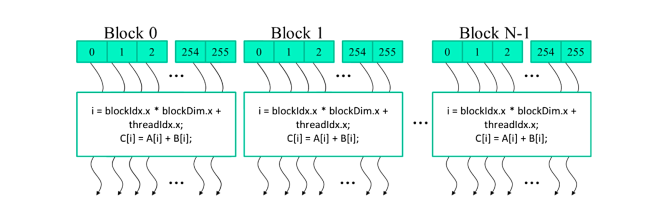
\includegraphics[width=\textwidth]{imagenes/graf_threads_blocks.png}
\end{frame}

\begin{frame}
    \frametitle{Estrategias e implementación}
    \begin{itemize}
        \item Un seed por thread
        \item Un fotón por thread
        \item heats en unified memory
    \end{itemize}
\end{frame}

\begin{frame}
    \frametitle{Estrategias e implementación}
    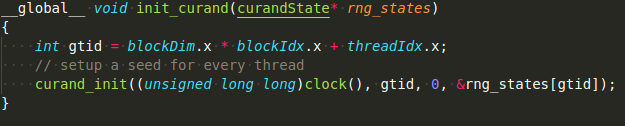
\includegraphics[width=\textwidth]{imagenes/code1.png}
\end{frame}

\begin{frame}
    \frametitle{Estrategias e implementación}
    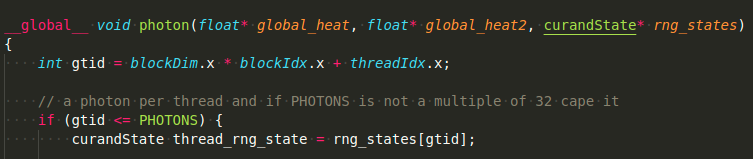
\includegraphics[width=\textwidth]{imagenes/code2.png}

\end{frame}

\begin{frame}
    \frametitle{Estrategias e implementación}
    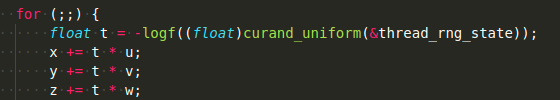
\includegraphics[width=\textwidth]{imagenes/code3.png}

\end{frame}

\begin{frame}
    \frametitle{Estrategias e implementación}
    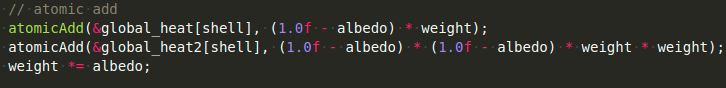
\includegraphics[width=\textwidth]{imagenes/code4.png}

\end{frame}

\begin{frame}
    \frametitle{Estrategias e implementación}
    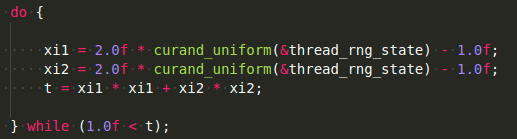
\includegraphics[width=\textwidth]{imagenes/code5.png}

\end{frame}

\begin{frame}
    \frametitle{Estrategias e implementación}
    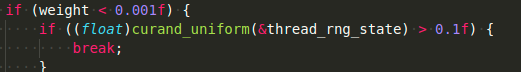
\includegraphics[width=\textwidth]{imagenes/code6.png}

\end{frame}

\begin{frame}
    \frametitle{Optimización al kernel}
    \begin{itemize}
        \item Arrays heat de memoria \_\_shared\_\_ 
    \end{itemize}
\end{frame}

\begin{frame}
    \frametitle{Optimización al kernel}
    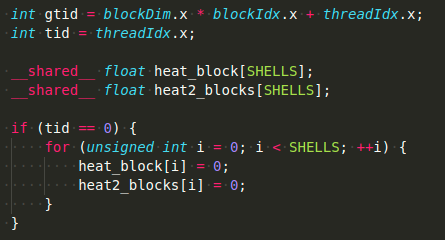
\includegraphics[width=\textwidth]{imagenes/code7.png}
\end{frame}

\begin{frame}
    \frametitle{Optimización al kernel}
    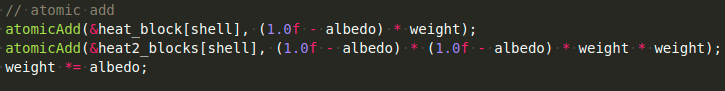
\includegraphics[width=\textwidth]{imagenes/code8.png}
\end{frame}

\begin{frame}
    \frametitle{Optimización al kernel}
    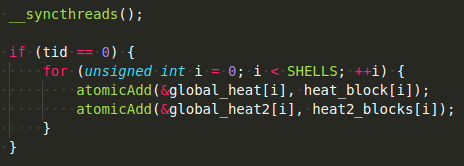
\includegraphics[width=\textwidth]{imagenes/code9.png}
\end{frame}

\begin{frame}
    \frametitle{Optimización al kernel}
    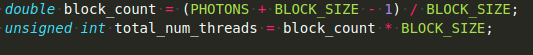
\includegraphics[width=\textwidth]{imagenes/code10.png}
\end{frame}

\begin{frame}
    \frametitle{Comparación con el resto de los labs}
    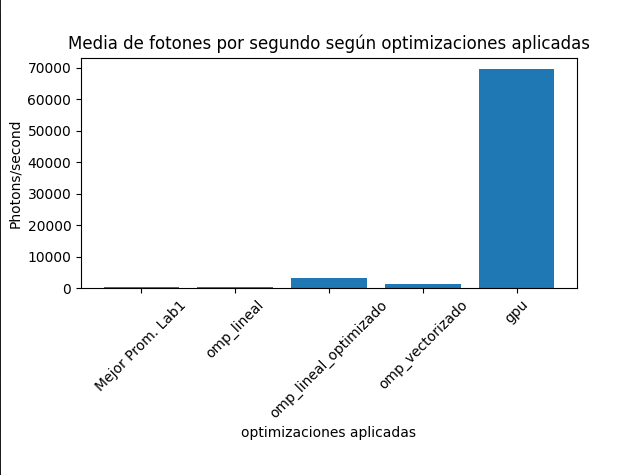
\includegraphics[width=\textwidth]{imagenes/media_opt_gpu.png}
\end{frame}

\begin{frame}
    \frametitle{Scaling}
    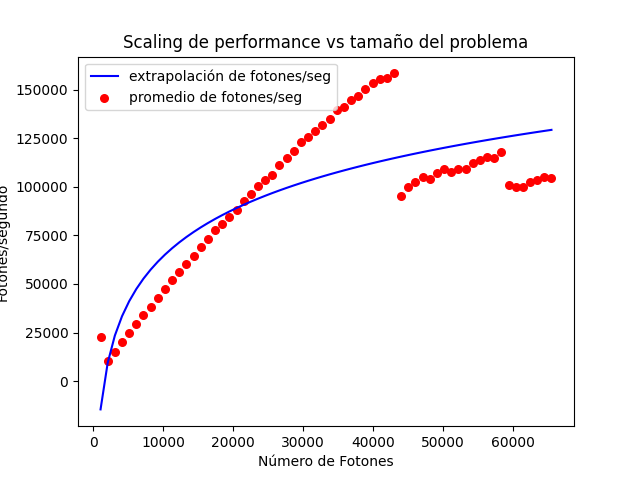
\includegraphics[width=\textwidth]{imagenes/scaling_gpu.png}
\end{frame}

\begin{frame}
    \frametitle{Posibles mejores}
    \begin{itemize}
        \item Uso de arrays a nivel de warp
        \item Escalar el problema
    \end{itemize}
\end{frame}

\end{document}